\chapter{Umsetzung} %Should be roughly 18pages
\label{kap:umsetzung}
\minitoc\pagebreak
% Erst JIRA Stories dann Datenmodell oder andersrum?
% Benötigtes Modell, dann stories, dann umsetzung
% Added new Data models like cpr, shocks, nibp!! as subsections!
% Viele Sachen Parallel...

\section{Technische Aspekte}
\label{sec:tech}
Zu Beginn der Umsetzung gilt es vorab diverse technische Aspekte zu analysieren und im Laufe der Entwicklung zu berücksichtigen.
Hierzu gehören beispielsweise die Schnittstelle und der daraus resultierende Export der Daten oder die Haltung der Daten in einer Datenbank.
Dies ist eine essentielle Basis, damit eine effiziente und angemessene Datengrundlage für die anschließend entwickelten Dashboards und Auswertungen zur Verfügung steht.

Dabei ist es bezüglich der Flexibilität und Unabhängigkeit von Vorteil , dass die Daten und der entsprechende Export nicht ausschließlich für die hier verwendete Technologie Qlik Sense abgestimmt und entwickelt werden.
Auch andere Software-Lösungen, Drittanbieterprogramme oder Business-Intelligence-Werkzeuge sollen die Daten und den neuen Export von \gls{ANALYSE} zur Auswertung verwenden können, damit eine gewisse Freiheit und keine absolute Abhängigkeit an einer Technologie entsteht.

\subsection{Schnittstelle \acrlong*{ANALYSE} und Qlik Sense} %StandDerTechnik??
\label{sub:schnittstelle}
Qlik Sense bietet eine Reihe an möglichen Datenverbindungen oder sogenannten \glqq Konnektoren\grqq.
Diese sind je nach Verbindungstyp vorgefertigte Module, welche die Verbindung zu gängigen Datenbanken oder anderen Quellen vereinfachen sollen.
Es können Daten aus lokalen Dateien wie CSV-, Excel- oder XML-Dateien, Datenbanken oder mittels standardisierten Schnittstellen geladen werden.
\bildbreit
{konnektoren}
{Qlik-Konnektoren zur Einrichtung von Datenverbindungen zu Datenbanken oder Schnittstellen}
{Qlik-Konnektoren für Datenverbindungen }

In Abbildung \ref{fig:konnektoren} sind die möglichen Datenbank- oder Schnittstellen-Konnektoren aufgelistet, wie beispielsweise \glqq MongoDB\grqq, \glqq Oracle\grqq, \glqq Microsoft SQL Server\grqq{} oder \glqq REST\grqq.

Da (wie in \ref{sub:StandTEchnikAnalyse} beschrieben) hinter \gls{ANALYSE} eine MongoDB-Datenbank steht, wäre der entsprechende Konnektor eine Möglichkeit, um die Einsatzdaten in Qlik bereitzustellen.
Allerdings befindet sich dieser zum einen in einem Beta-Zustand, zum anderen widerspricht dies der Philosophie, einen universellen Export der Daten zu bieten, da nicht jede Technologie einen Konnektor zur MongoDB hat. 

Ein weiterer Faktor ist außerdem die Sicherheit der Daten.
Gewährt man einem Drittprogramm und damit mehreren Nutzern den direkten Zugriff auf eine Datenbank, entstehen gewisse Risikofaktoren, welche die Sicherheit des Systems gefährden.
Schließlich liegen gegebenenfalls personenbezogene Daten in der Datenbank \ref{sec:rechtlich} oder Daten, welche gewisse Entscheidungen zur Folge haben.
Eine mögliche unkontrollierte Manipulation dieser Information sollte vermieden werden.

Demnach sollte es eine Schnittstelle von \gls{ANALYSE} geben, welche die Daten kontrolliert bereitstellt.
Eine sehr geeignete Technologie hierfür ist eine \gls{REST}ful API.
Vorteile hiervon sind laut Steimle \cite[2.3]{Steimle.2014} und Tilkov \cite[1.1]{Tilkov.2011} unter anderem:
\begin{itemize}
\item Die Kopplung der Systeme wird so gering wie möglich gehalten. 
Durch die homogen entwickelte Schnittstelle sind alle möglichen Vorgänge definiert und deren Aufruf spezifiziert.
So werden ungewollte Zugriffe auf die Daten in der Datenbank vermieden
\item Die gewollte Interoperabilität wird stark gewährleistet, da \gls{REST} auf gängigste Standards setzt. 
Dadurch können die meisten derzeitigen und zukünftigen Systeme mit dieser Technologie kommunizieren.
\item Die Wiederverwendung ist durch die einmalige Definition der Schnittstelle sehr hoch.
\item Die Skalierbarkeit und die daraus resultierende Performance kann mit \gls{REST} auch bei häufigen und großen Anfragen gewährleistet werden.
\end{itemize}

Außerdem bietet \gls{REST} die Möglichkeit, Zugriffe nur mit einer Authentifizierung durchzuführen.
Dies spiegelt das derzeitige Benutzergruppen-Konzept von den \cweb-Produkten sehr gut wider.

Mit diesen auf die Anforderungen passenden Vorteilen wurde sich für eine Schnittstelle der \gls{REST}-Technologie entschieden.
\gls{ANALYSE} besitzt bereits ein \gls{REST}-Interface, allerdings hat dieses bis dato einen anderen Zweck.

\subsection{Export der Daten} %subsub?
\label{sub:export}
Nach Festlegung der Technologie für die zukünftige Schnittstelle in \ref{sub:schnittstelle} werden nun die weiterführenden Schritte geplant und umgesetzt.
Das bestehende \gls{REST}-Interface soll demnach um einen Endpoint erweitert werden, welcher die Daten, respektive die \gls{MM} von allen Einsätzen eines \gls{ANALYSE}-Servers exportiert.

Dabei soll von Vornherein eine Authentifizierung notwendig sein, um die entsprechenden Daten des Servers zu erhalten.
Hierfür wird zunächst das \glqq Baisc Authentication\grqq-Verfahren als HTTP-Authentifizierung verwendet. 
Dabei können die angelegten Benutzer im aktuellen Mandanten von \gls{ANALYSE} sich mit dem entsprechenden Passwort im Header des \gls{REST}-Calls authentifizieren.

\subsubsection{Erstes Exportformat}
\label{subsub:1stexport}
Der erste Ansatz für einen solchen Export war ein zweistufiger Prozess:
\begin{enumerate}
\item Ein Export wird angestoßen, welcher von allen vorhandenen Einsätzen die jeweilige \gls{UUID} im Response-Body zurückgibt.
\end{enumerate}

Dieser erste Schritt wird mit der HTTP-Methode \glqq GET\grqq{} ausgeführt.
Im Header der Anfrage ist die in \ref{sub:export} genannte Authentifizierung sowie das entsprechende Format der Anfrage, der \glqq content-type\grqq, festgelegt.

Als Parameter können außerdem die maximale Anzahl an UUIDs sowie eine \gls{CQL}-Abfrage mitgegeben werden.
Ein Beispiel eines solchen Befehls kann dabei so aussehen:

\code{-GET http://corpsrv5009:8080/v3/missionlist/missions/query/start?cql=hasShocks\& batchsize=2000}
Code oder Bild (mit Zahlen)?

Mit diesem Befehl werden beispielsweise alle UUIDs der Einsätze geladen, die mindestens eine Defibrillation vorzeigen. 
Mittels des Parameters \glqq batchsize\grqq{} wird die Antwort auf maximal 2000 Einsätze beschränkt.
Das zurückgelieferte Objekt ist dabei ein JSON-Objekt mit einem Key-Value-Paar \code{"'uuids"': []}, welches als Wert die vielen \gls{UUID}s in einem Array speichert.

\begin{enumerate}[resume]
\item Im zweiten Schritt werden mit den erhaltenen UUIDs die weiterführenden \gls{MM} der Einsätze angefordert.
\end{enumerate}

Im Gegensatz zum ersten Schritt wird hierbei die HTTP-Methode \glqq POST\grqq{} verwendet.
Dies hat den Hintergrund, dass so die möglicherweise enorme Anzahl an \gls{UUID}s in den Request-Body des Befehls geschrieben werden können, statt in die URL.
Demnach wird der Body der Anfrage mit dem zuvor erhaltenen JSON-Objekt, sowie den gewünschten \gls{MM} beschrieben.
Auch hier ist wieder eine Basic-Authentifizierung notwendig, damit kein unerlaubter Zugriff auf die Daten erfolgen kann.\todo{Dark or White Theme?}

\begin{figure}[ht]
\begin{subfigure}{.5\linewidth}
  \centering
  % include first image
  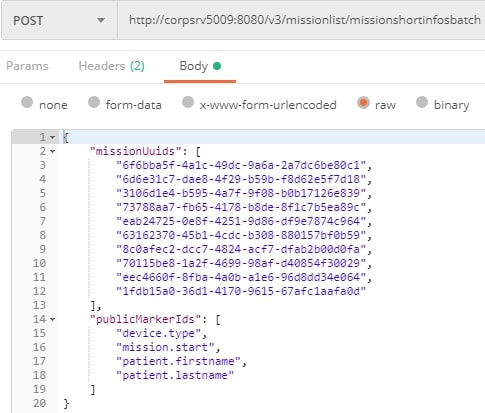
\includegraphics[width=.95\linewidth]{img/exRequestW}  
  \caption{Beispiel des POST-Requests}
  \label{fig:request}
\end{subfigure}
\begin{subfigure}{.5\linewidth}
  \centering
  % include second image
  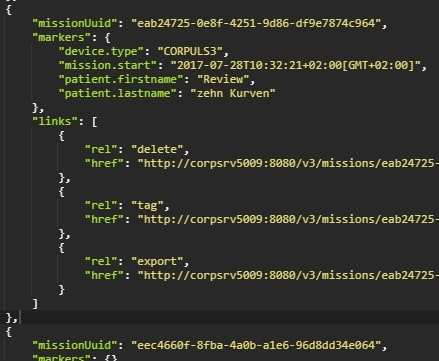
\includegraphics[width=.95\linewidth]{img/exResponse}  
  \caption{Auszug der Antwort auf den POST-Request}
  \label{fig:response}
\end{subfigure}
\caption[Beispiel einer Anfrage und Antwort der POST-Methode]{Beispiel einer Anfrage und Antwort der POST-Methode, um die \gls{MM} der im Body angegebenen Einsätze zu erhalten}
\label{fig:fig}
\end{figure}

In Abbildung \ref{fig:request} ist ein solcher POST-Request zu sehen.
In der URL wird der entsprechende \gls{ANALYSE}-Server adressiert, um auf die Daten der einzelnen Einsätze zugreifen zu können.
Im Body werden hierbei die aus Schritt 1 angeforderten Objekte eingefügt: \glqq missionUuids\grqq{} und \glqq publicMarkerIds\grqq.

Als Antwort erhält man mehrere \glqq Missions-Objekte\grqq{}, welche die \gls{UUID} und die entsprechenden \gls{MM} mit den individuellen Werten einer Mission enthält.
Ein Auszug einer solchen Antwort ist in \ref{fig:response} zu sehen.
Des Weiteren gibt es ein \glqq Link-Objekt\grqq{}, mit welchem ein Einsatz gelöscht, exportiert oder verändert werden kann. 

Positiv an diesem Export ist, dass die Anzahl der exportierten bedingt festgelegt werden kann.
Allerdings wird dieses Schema bei größeren Datenmengen, was genau das Ziel bei den Auswertungen ist, zu Problemen führen.
So kann das entsprechende Objekt mit den Einsatz-\gls{UUID}s sehr groß werden und beim kopieren und einfügen in den darauffolgenden Request-Body Schwierigkeiten bereiten.
Auch der damit resultierende große POST-Befehl ist keine optimale Umsetzung.

Aus diesem Anlass muss dieses Export-Format neu überdacht und für große Datenmengen optimiert werden.

\subsubsection{Überarbeitetes Export-Format}
\label{subsub:ueberarbeutetesformat}
Der Hauptaspekt beim neuen Entwurf der Export-Schnittstelle war das effiziente und sichere Umgehen mit großen Datenmengen.
Hierfür muss ein anderer als der zweistufige, in \ref{subsub:1stexport} beschriebene Prozess, entwickelt werden.

\todo{Alternativen: Direkt auf Platte, Anstoßen und direkt Ergebnis erhalten oder eben Anfrage und später fertige Datei\\
Warum letzteres: Nie Timeout und sicherheit(auth) und universell}
%\lipsum*[104]

Letztendlich wurde sich für ein/das Konzept mit den folgenden möglichen Schritten entschieden:
\begin{enumerate}
\item Die Generierung eines Exports anstoßen
\item Alle angeforderten Exports auflisten
	\begin{enumerate}
	\item Details zu einem explizitem Export bekommen
	\item Bestimmten Export löschen
	\end{enumerate}
\item Objekt/Datei mit allen Einsätzen und zugehörigen Daten mittels eigenem Link abrufen
\end{enumerate} 

Zum Erhalt der Export-Datei sind alle drei Schritte notwendig, 2a) \& b) sind als optionale Funktionen verfügbar.
Auch hier ist bei allen Vorgängen eine entsprechende Authentifizierung notwendig, um entsprechende Aktionen anzustoßen oder Informationen zu erhalten.

\begin{enumerate}
\item \code{-POST http://10.97.3.109:8080/v3/exports}
\end{enumerate}
Der erste Vorgang ist hierbei der POST-Befehl, der auf dem entsprechenden Server die Generierung eines neuen Exports anstößt.
Dabei werden alle verfügbaren Einsätze mit allen vorhandenen \gls{MM} exportiert.
Dies wurde so festgelegt, da der Anwender in der Regel mit einem solchen Export alle Missionen erhalten möchte.
Die Erweiterung um einen ressourcensparenden \glqq Incremental Load\grqq{} wird in \ref{sub:incremental} weiter betrachtet.

\begin{enumerate}[resume]
\item \code{-GET http://10.97.3.109:8080/v3/exports}
\end{enumerate}

Daraufhin ist es mit dem zweiten Schritt möglich, alle angestoßenen, laufenden und fertigen Exports aufzulisten.
Dabei wird mit der identischen URL die GET-Methode ausgeführt.
Hierbei werden pro Export zusätzliche Informationen bereitgestellt (siehe Abbildung \ref{fig:exportListWide}): 

%Die Start-Zeit (\glqq startTime\grqq) als UTC-Zeitstempel in Millisekunden, wann dieser Export angestoßen wurde.
%Analog der End-Zeitpunkt (\glqq endTime\grqq) wann dieser Export fertiggestellt wurde, die Anzahl Missionen, der jeweilige Status, ob angestoßen, laufend oder fertig, Links für weitere Optionen sowie die ID des Exports.

\begin{itemize}
\item Start-Zeit (\glqq startTime\grqq): UTC-Zeitstempel in ms, wann dieser Export angestoßen wurde
\item End-Zeit (\glqq endTime\grqq): UTC-Zeitstempel in ms, wann dieser Export fertiggestellt wurde
\item Anzahl der exportierten Einsätze (\glqq missions\grqq)
\item Status, ob angestoßen, laufend oder fertig
\item Links zu den weiteren Optionen
\item Die ID des Exports
\end{itemize}

\bild
{exportListWide}
{12cm}
{Antwort des Servers - Auszug der Auflistung von zwei fertiggestellten Exports als JSON-Objekte}
{Auflistung von Exports}

Demnach werden angeforderte Exports für eine ausgewählte Dauer gespeichert, was für unterschiedliche Szenarien ein Vorteil sein kann.
Auch die Möglichkeit, einen angeforderten Export wieder zu löschen ist eine hilfreiche Funktion, welche einen Server entlasten kann, sollten beispielsweise zu viele Exporte angefordert worden sein.
Der Status ist ebenfalls eine nützliche Information, welche den Empfang des fertigen Exports an ein \gls{BI}-Werkzeug erleichtern und garantieren kann.

\begin{enumerate}[resume]
\item \code{-GET http://10.97.3.109:8080/v3/exports/\{EXPORT\_ID\}/file}
\end{enumerate}

Im letzten Schritt wird der entsprechend bereitgestellte Link mitels GET-Methode aufgerufen.
Daraufhin erhält der Anwender den gesamten Export mit allen Einsätzen und den dazugehörigen \gls{MM} im JSON-Format. 
Ein Beispiel dieser Antwort ist Abbildung \ref{fig:exportFile} zu entnehmen.
\bild
{exportFile}
{9cm}
{Auszug des Exports mit allen Einsätzen und dazugehörige \gls{MM}}
{Auszug des Exports}

Der größte Vorteil dieses neuen Formats ist der Umgang mit großen Datenmengen.
Es müssen keine riesigen Objekte kopiert und eingefügt oder an eine andere Stelle weitergeleitet werden. 
Auch sind keine weiteren umständlichen Parameter notwendig. \\
Die URL wurde mit dem Schema \\
\colorbox[RGB]{240,240,240}{\texttt{http://\{SERVER\_IP\}/v3/exports}} \\
standardisiert, sodass keine unterschiedlichen URLs mit vielen optionalen Parametern wie in \ref{subsub:1stexport} notwendig sind.
Lediglich beim finalen Anfordern der Export-Datei muss die Standard-URL um \\
\colorbox[RGB]{240,240,240}{\texttt{http://\{SERVER\_IP\}/v3/exports\textcolor{red}{/\{EXPORT\_ID\}/file}}} \\
erweitert werden. 

\subsection{Erweiterung um neue Datenobjekte} %tiefgreifendere? Daten}
\label{sub:erweiterung}
Im Rahmen der \fullref{kap:anforderungsanalyse} kamen bereits erste Fragestellungen zum Vorschein, welche mit den bisherig zur Verfügung stehenden Daten nicht beantwortbar waren.
Im darauffolgenden Laufe der \fullref{kap:konzept} haben sich diverse weitere Problematiken und fehlende Daten für aussagekräftige Auswertungen bestätigt.

So ist beispielsweise eine ausdrucksvolle Analyse zur Drucktiefe in der Reanimation über mehrere Missionen nicht in der Form umsetzbar, wie sie sinnvoll und gewünscht wäre.
Hier ist lediglich der Mittelwert der Drucktiefe von der gesamten Reanimation vorhanden.
Eine inhaltsreiche Auswertung, auch beispielsweise mit Veränderungen innerhalb der Reanimation, sind schlicht nicht möglich.
In diesem Stil gibt es weitere, für Auswertungen sinnvolle Daten, die derzeit gar nicht, oder nur als stark aggregierte Werte vorhanden sind.
Eine Analyse der potentiell verfügbaren Daten ergab folgende Bereiche (Auszug im Anhang \ref{anhangProbleme}):  %Markante Beispiele sind:
\begin{description}
\item [Reanimationsqualität]\hfill \\
Drucktiefe \& -frequenz, Anzahl Kompressionen, Pausenzeiten und \gls{CCF}
\item [Defibrillationen]\hfill \\
Zeitpunkt, Energie, Impedanz, Modus und Pausenzeiten der einzelnen Defibrillationen
\item [\gls{NIBD}]\hfill \\
Zeitpunkt, Modus, Dauer , Patiententyp, Systole, Diastole \& mittlerer arterieller Druck der einzelnen Messungen
\item [Vitalparameter und Trends]\hfill \\
Die Werte aller Vitalparameter zu einem bestimmten Zeitpunkt
\item [Technische- und Patienten-Alarme]\hfill \\
Wann sind welche Patientenalarme mit welchen Alarmgrenzen aufgetreten? \\
Welche technischen Alarme treten zu welcher Zeit auf?
\item [Events]\hfill \\
Welche Events treten wann mit welchen Parameter-Werten auf?
\end{description}

Mit diesen Daten wären weit detailliertere und tiefgreifendere Auswertungen möglich. 
Dabei würde vor allem die explorative Datenanalyse (siehe S.\pageref{subsub:datenanalyse}, \ref{subsub:datenanalyse}) profitieren.

Diese erfordern jedoch eine Überlegung des späteren Datenmodells, da diese das Konzept von multidimensionale Daten darstellen.
Demnach gibt es einen Datensatz mit \textit{n} Einsätzen, wovon jeder Einsatz eine Anzahl \textit{m} Kompressionen, Defibrillationen, Messungen, Alarme und weiteres haben kann.
Einen Entwurf für ein passendes Datenmodell ist in Abbildung \ref{fig:ersterVorschlagDatenmodellC} zu sehen.

Auf Basis dieser Analyse und der herausgefundenen potentiellen neuen Datenquellen werden Anforderungen formuliert und mit der Entwicklungsabteilung kommuniziert, damit diese Daten zur Auswertung bereitstehen können.

\subsubsection{Entwurf für ein Datenmodell}
\label{subsub:datenmodell}
Um die Anforderung, weitere Daten aus den bisherigen Einsätzen auszulesen gerecht zu werden, muss vorab ein geeignetes Datenmodell entworfen werden.
Dieses muss die daraus resultierende Multidimensionalität unterstützen und eine konfliktfreie Umgebung schaffen.
Dabei sollen jedoch so viele Daten wie möglich miteinander kombiniert werden können, damit ein umfassendes exploratives und konfirmatives Analysieren der vorliegenden Daten möglich ist.

Zuvor gab es lediglich die Tabelle \glqq Missions\grqq{}, welche pro Zeile einen Einsatz ablegt und in den dazugehörigen Spalten die Werte zu den entsprechenden \gls{MM}.
Ein Auszug aus hieraus ist in Tabelle \ref{tbl:missions} zu sehen.

\begin{table}[htb]
\centering
%\resizebox{\textwidth}{!}{%
\begin{tabular}{|l|l|l|l|l|}
\hline
\textbf{mission.uuid}   & \textbf{mission.start} & \textbf{hasReanimation} & \textbf{device.type} & \textbf{...} \\ \hline
b14f790f-{[}...{]}863f3 & 2016-08-27T12:13:07    & true                    & corpuls3             & ...          \\ \hline
d7276b88-{[}...{]}2da61 & 2016-09-29T21:02:30    & false                   & corpuls1             & ...          \\ \hline
\end{tabular}%
%}
\caption[Aktuelle Export-Tabelle]{Auszug aus der Tabelle, wie sie im aktuellen Export maximal zur Verfügung steht}
\label{tbl:missions}
\end{table}

Ein geeignetes Datenmodell, welches die mehrdimensionalen Daten einbindet und unterstützt, wurde entworfen und ist in Abbildung \ref{fig:ersterVorschlagDatenmodellC} zu erkennen.
Hierbei wurden die in \ref{sub:erweiterung} genannten neuen Datenquellen hinzugefügt, sodass beispielsweise neue Tabellen zu \gls{CPR}- oder Defibrillationsdaten zu sehen sind.

\bildbreit
{ersterVorschlagDatenmodellC}
{Visualisierung für den Entwurf eines neuen Datenmodells mit mehrdimensionalen Objekten}
{Visualisierung des neuen Datenmodells mit mehrdimensionalen Objekten}

Dabei wurde darauf geachtet, dass keine zirkulären Referenzen entstehen, welche unter anderem bei der gleichen Benennung mehrerer Spalten vorkommen.
Dies wurde präventiv mit einem Präfix der jeweiligen Datenquelle verhindert.
Auch erleichtert dies das spätere Erstellen von Dimensionen oder Kennzahlen, da eine eindeutige Benennung vorhanden ist.

Auch ein gemeinsamer Primärschlüssel sollte in allen neuen Datentabellen vorhanden sein, damit eine Beziehung herrscht.
Hierfür wurde die \gls{UUID} verwendet, da diese garantiert in jedem Einsatz vorhanden und bereits eindeutig ist.
Damit ist gewährleistet, dass theoretisch jeder Datenpunkt mit jedem anderen Datenpunkt verknüpft werden kann, auch wenn nur ein geringer Teil aller Verknüpfungen sich als sinnvoll erweisen wird. 


%\subsection{Incremental Load?}
\subsubsection{Erstellen von Anforderungen für neue Datenquellen} %(als User Stories in JIRA)}
\label{subsub:stories}
Damit die im vorherigen Kapitel herausgefundenen Datenquellen für Auswertungen bereitstehen, muss zunächst deren Extrahierung aus den Einsatzdaten implementiert werden. 
Weiter steht der Export, beziehungsweise das Hinzufügen dieser neuen Daten in den bestehenden, überarbeiteten Export an.

Hierfür wird der bestehende Prozess der Entwicklungsabteilung angewandt, damit eine entsprechende Implementierung im SCRUM-Verfahren möglich ist.
Demnach wird für eine neue Anforderung eine \glqq Story\grqq{} im Projekt- und Aufgabenmanagement-Tool \glqq Jira\grqq{} angelegt.
Diese Story wird einem übergeordneten \gls{Feature} oder \glqq Epic\grqq{} zugeordnet.
So werden beispielsweise dem Feature \glqq \gls{BI} Dashboard\grqq{} alle zugehörigen Storys zugeordnet, wie in einem Auszug davon in Abbildung \ref{fig:jiraEpic} zu sehen ist.
\bild
{jiraEpic}
{12cm}
{Grafische Visualisierung der zugehörigen Storys vom Feature \glqq \gls{BI} Dashboard\grqq{} in Jira}
{Visualisierung der zugehörigen Storys vom Feature BI-Dashboard in Jira}

Weiter muss eine Story laut SCRUM die \glqq Definition of Ready\grqq{} erfüllen, damit sie in den Sprint mit eingeplant werden darf.
Diese soll garantieren, dass unter anderem eine aussagekräftige Beschreibung oder Abnahmekriterien vorhanden sind.
Dementsprechend müssen die erstellten Storys gewisse Qualitätsmerkmale vorweisen, damit sie umgesetzt werden können.

Für das Extrahieren und Exportieren von einem neuen Datenobjekt ist es daher sinnvoll, die geforderten Informationen so detailliert wie möglich darzulegen.
Hierfür ist das vorab in \ref{subsub:datenmodell} entwickelte Datenmodell ein hilfreiches Mittel, um die Storys präzise beschreiben zu können.

\begin{table}[hbt]
\centering
\resizebox{\textwidth}{!}{%
\begin{tabular}{ll|l|l|l|l|l|l|}
\cline{3-8}
                                       &                       & \multicolumn{6}{c|}{\textbf{trend.}}                                                                                                                                              \\ \cline{3-8} 
                                       &                       &                       & \multicolumn{5}{c|}{\textbf{cpr.}}                                                                                                                        \\ \hline
\multicolumn{1}{|l|}{\textbf{}}        & \textbf{mission.uuid} & \textbf{minute} & \textbf{pauses.sum} & \textbf{comp.sum} & \textbf{depth.avg} & \textbf{rate.avg} & \textbf{ccf} \\ \hline
\multicolumn{1}{|l|}{\textbf{Type}}    & uuid                  &                       & int                           & int                                 & float                        & float                       & float                  \\ \hline
\multicolumn{1}{|l|}{\textbf{Unit}}    &                       &                       & s                             &                                     & cm                           & 1/min                       &                        \\ \hline
\multicolumn{1}{|l|}{\textbf{Example}} & sd84-[...]-k9s4s      & 3                     & 13                            & 91                                  & 5.31                         & 112                         & 0.82                   \\ \hline
\end{tabular}%
}
\caption[Gefordertes Exportformat am Beispiel der CPR-Daten]{Auf Basis des entworfenen Datenmodells erstellte Tabelle für das geforderte Export-Format am Beispiel von \gls{CPR}-Daten}
\label{tbl:export}
\end{table}

Für eine solche detaillierte Beschreibung der Story wurde unter anderem eine Tabelle \ref{tbl:export} angelegt.
In dieser Darstellung sind bereits viele Aspekte festgelegt.
So ist beispielsweise die Namensgebung an die bisherige Nomenklatur der \gls{MM} angelehnt, sodass eine innere Konsistenz herrscht.
Auch der jeweilige Datentyp oder die Einheit ist bereits festgelegt, damit ein einheitliches Format der Daten gewährleistet ist.

Die Einheit ist insofern von großer Bedeutung, da diverse Daten in verschiedenen Einheiten gespeichert werden können.
So kann etwa die CO2-Konzentration der Ausatemluft in Millimeter-Quecksilbersäule (mmHg) oder Kilopascal (kPa) gemessen und gespeichert werden.
Damit in der späteren Auswertung keine unterschiedlichen Einheiten vermischt werden, wird in Tabelle \ref{tbl:export} eine Standard-Einheit für den Export festgelegt.

Auch der Aggregierungsgrad wird hier beschrieben, indem die Daten für eine Minute aggregiert werden sollen.
Dies resultierte aus mehreren Diskussionen mit Entwicklern, Produktmanager und Stakeholdern, da die Speicherung von jeder einzelnen Kompression mit ihren vorliegenden Daten auf lange Sicht zu einem Speicher- und Performanceproblem führen könnte.
Dennoch ist es für die Anwender eine deutliche Verbesserung der Auswertungsmöglichkeiten.

Ein Beispiel für exemplarische Daten wird ebenfalls hinzugefügt, damit letzte Unklarheiten zu Feldern oder Datentypen beseitigt werden.
Dieser Prozess wird analog mit allen neu geforderten Objekten (siehe Abbildung \ref{fig:ersterVorschlagDatenmodellC}) durchgeführt. Anhang\ref{AnhangJiraStories?}

\subsubsection{Festlegen des Export-Formats}
Im Zuge der Bereitstellung der neuen Datenobjekte wurde im vorigen Kapitel mittels Beschreibung der Anforderungen und ergänzenden Tabellen das gewünschte Format festgelegt.
Im Laufe der Implementierung gibt es diverse Diskussionen und Abstimmungen mit den Entwicklern und Stakeholdern, wie der finale Export aussehen soll.
Dies geschieht im Zuge der \glqq Sprints\grqq{} in mehreren Zyklen, wird jedoch für die bessere Lesbarkeit dieser Arbeit in diesem Unterkapitel zusammengefasst.

Vorab ist anzumerken, dass im zeitlichen Rahmen dieser Arbeit und unter Berücksichtigung von anderen Entwicklungsprojekten eine Priorisierung des Product-Owners vorgenommen werden musste.
Dabei sind drei der sechs geforderten neuen Datenobjekte aus Abbildung \ref{fig:ersterVorschlagDatenmodellC} für die Erweiterung des Exports  geplant: \gls{CPR}-, \gls{NIBD}- \& Defibrillations-Daten.

Demnach soll es drei optionale neue JSON-Objekte in der Antwort des Servers (siehe Abbildung \ref{fig:exportFile}) geben.
Hier wurden vorab Überlegungen getätigt, wo die entsprechenden neuen Daten hierarchisch zugeordnet werden.
Dabei gibt es generell zwei Optionen:
Die neuen Objekte dem \glqq markers\grqq-Objekt unterordnen (Abbildung \ref{fig:marker}), oder direkt unterhalb des \glqq mission\grqq-Objektes als zweiten Kindknoten (\ref{fig:mission}).

\begin{figure}[ht]
\begin{subfigure}{.5\linewidth}
  \centering
  % include first image
  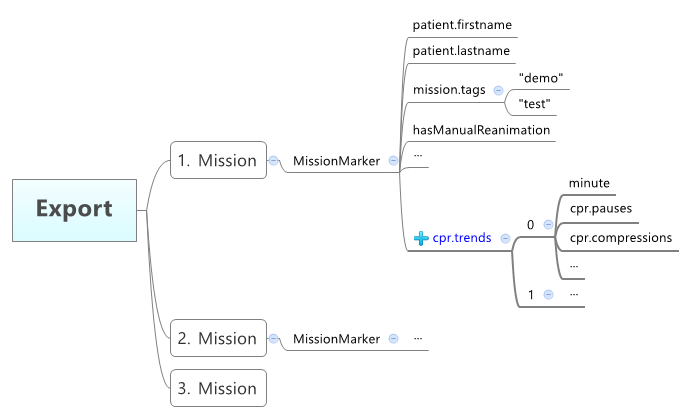
\includegraphics[width=.95\linewidth]{img/format1}  
  \caption{CPR-Objekt unterhalb des \glqq markers\grqq-Objekt}
  \label{fig:marker}
\end{subfigure}
\begin{subfigure}{.5\linewidth}
  \centering
  % include second image
  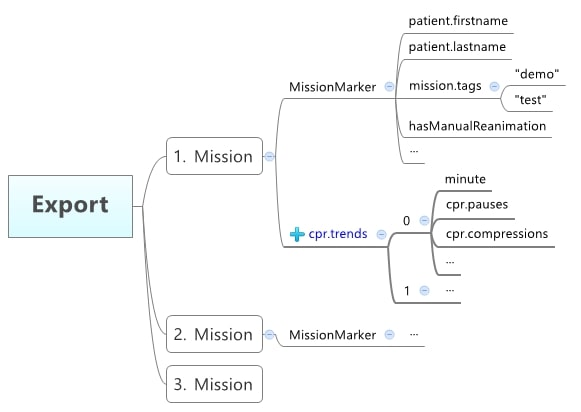
\includegraphics[width=.95\linewidth]{img/format2}  
  \caption{Neues Objekt neben dem \glqq markers\grqq-Objekt}
  \label{fig:mission}
\end{subfigure}
\caption[Beispiel einer Anfrage und Antwort der POST-Methode]{Schematische Darstellung der Erweiterung des Exports am Beispiel vom CPR-Objekt}
\label{fig:tree}
\end{figure}

Da es sich um eigenständige neue Objekte unabhängig von den \gls{MM} handelt, wurde sich für die Variante in Abbildung \ref{fig:mission} entschieden.
Demnach können nun die Objekte \glqq trend.cpr\grqq, \glqq shock.details\grqq{} und \glqq nibp.details\grqq{} in einem Missions-Objekt vorhanden sein.
Ein Beispiel hierfür ist in Abbildung \ref{fig:exportNewObj} zu sehen.

\bild
{exportNewObj}
{9cm}
{Neue JSON-Objekte (hier \glqq trend.cpr\grqq{} \& \glqq shock.details\grqq{}) neben den \glqq markes\grqq{} innerhalb eines Missions-Objektes des Exports}
{Neue JSON-Objekte innerhalb eines Missions-Objektes des Exports}

%(Diese zwei Optionen sind in Abbildung \ref{fig:tree} schematisch dargestellt.
%Dabei ist in \ref{fig:marker} das Schema mit der Unterordnung unterhalb des \glqq markers\grqq-Objekt visualisiert.
%In \ref{fig:mission} ist das \gls{CPR}-Objekt unterhalb der ersten Mission als zweites Kindobjekt neben den \glqq markers\grqq angelegt.)

Des Weiteren wurde entschieden, die neuen Objekte nur zu exportieren, wenn auch tatsächlich Daten hiervon vorhanden sind.
Bei dem \gls{CPR}-Objekt gibt es hierbei eine Besonderheit, da dieses als zeitliches Objekt mit Trenddaten anzusehen ist.
Dadurch gibt es immer Daten ab Minute 0, auch wenn beispielsweise die erste Kompression erst in Minute zwölf stattfand.
Dies soll garantieren, dass eine kontinuierliche Zeitskala gegeben ist, die auch mit anderen Trenddaten vergleichbar ist.
Für eine Vergleichbarkeit von Reanimationen untereinander ist diese Form der Daten nicht geeignet. 
In \ref{subsub:weitereFelder} wird eine Lösung erarbeitet, die dies zusätzlich ermöglichen soll.

Bei den \gls{NIBD}- \& Defibrillations-Objekten ist im Gegensatz zum CPR-Objekt nicht die Minute das führende Feld respektive Primärschlüssel, sondern die hochzählende Nummer der Messung oder der Schockabgabe.
Dadurch ist aufgrund der Objekorientierung eine Repräsentation der Wirklichkeit gegeben, da eine Messung oder eine Defibrillation ein abgeschlossenes Objekt darstellt.

%(json format cpr (siehe mails) (Fotos whiteboard als anhang?),)
%null values bei cpr trends

%% Vor Export?
%\subsection{Datenbankhaltung?}
%\subsubsection{Lasttests?}
%%dummydaten?


%\section{Datenmodell?}

\section{Erstellung der Qlik-App(s)}
\label{sec:erstellung}
%subsUnterschiedliche Apps?
\subsection{ETL-Prozess}
\label{sub:etl}

\subsubsection{Ladeskripte}
\label{subsub:scripts}

\subsubsection{Demo- und Testeinsätze herausfiltern}
\label{subsub:testfilter}

\subsubsection{Weitere manuell hinzugefügte Felder (ReaStart, Calendar, Test...)}
\label{subsub:weitereFelder}


\subsection{Datenmodell (hier oder eigene section?)}
\label{sub:datenmodell}

\subsection{Dimensionen}
\subsection{Kennzahlen}
\subsection{Verwendung von Erweiterungen?}
\subsection{Dashboards}
\subsubsection{Neue mögliche Visualisierungen durch Anforderungen Schocks, Nibp, Cpr}
test
\subsection{Umsetzung der Evaluierungsergebnisse (Auszug)}
\subsubsection{Zielgruppenunterschiedliche Startseiten}
\subsubsection{Lesezeichen?} %vlt so 10 Beispiel Lesezeichen
\subsubsection{Usability/Nutzerführung/Hilfetexte}
\subsubsection{Reduzierung Inhalt pro Arbeitsblatt}
\subsubsection{Weitere}
%subs testeinsätze filtern

\subsection{Einstellungen der Arbeitsblätter und Diagramme}
% (wie zB. Farben bei Auswahl beibehalten)
%CustomThemes?
%subs internationalisierung

% Aspekte vor Erstellung??
\section{Rechtliche Aspekte?}
\subsection{Datenschutz}
\subsection{Anonymisierung}


\section{Sonstige Aspekte?}
\subsection{Auslieferungsprozess?}
\subsection{Internationalisierung}
\subsection{Incremental Load?}
\label{sub:incremental}


\section{Evaluierung der Ergebnisse?}
%subs Usability-Tests?
